\documentclass[12pt,a4paper]{article}
\usepackage[utf8]{inputenc}
\usepackage[spanish,es-tabla]{babel}
\usepackage{geometry}
\usepackage{graphicx}
\usepackage{multirow}
\usepackage{tabularx}
\usepackage{mathptmx}
\usepackage{fancyhdr}
\usepackage{array}
\usepackage[table]{xcolor}
\usepackage{titlesec}
\usepackage{setspace}
\usepackage{microtype}
\usepackage{lastpage}
\usepackage{booktabs}
\usepackage{enumitem}
\usepackage{amsmath}
\usepackage{amsfonts}
\usepackage{amssymb}

\usepackage{float}
\usepackage{placeins}
\usepackage{tikz}
\usepackage{pgfplots}
\pgfplotsset{compat=1.17}
\usetikzlibrary{arrows.meta,positioning,shapes.geometric,calc}

\graphicspath{{images/}{../images/}{./}}

\geometry{
    top=4.7cm,
    bottom=2.5cm,
    left=2.5cm,
    right=2.5cm,
    headheight=3.9cm,
    headsep=0.4cm
}

\setstretch{1.15}
\setlength{\parindent}{0pt}
\setlength{\parskip}{0.45em}
\setlength{\tabcolsep}{4pt}

\titleformat{\section}
  {\normalfont\fontsize{12}{14.5}\bfseries}{\thesection.}{0.6em}{\uppercase}
\titlespacing*{\section}
  {0pt}{1.8ex plus 0.4ex minus 0.2ex}{0.6ex plus 0.2ex}

\titleformat{\subsection}
  {\normalfont\fontsize{11.5}{13.5}\bfseries}{\thesubsection.}{0.5em}{}
\titlespacing*{\subsection}
  {0pt}{1.4ex plus 0.3ex minus 0.1ex}{0.4ex plus 0.1ex}

\titleformat{\subsubsection}
  {\normalfont\fontsize{10.5}{12.5}\bfseries\itshape}{\thesubsubsection.}{0.4em}{}
\titlespacing*{\subsubsection}
  {0pt}{1.1ex plus 0.2ex minus 0.1ex}{0.3ex plus 0.1ex}

\newcolumntype{Y}{>{\centering\arraybackslash}X}
\newcolumntype{L}{>{\raggedright\arraybackslash}X}
\newcolumntype{C}{>{\centering\arraybackslash}X}

\definecolor{headerblue}{RGB}{26, 54, 93}
\definecolor{darkblue}{RGB}{43, 108, 176}
\definecolor{lightgraybg}{RGB}{248, 248, 248}
\definecolor{tableheader}{RGB}{232, 238, 246}
\definecolor{navyheader}{RGB}{0, 32, 96}
\definecolor{lineblue}{RGB}{0, 102, 204}
\definecolor{areablue}{RGB}{220, 236, 252}
\definecolor{lcsred}{RGB}{217, 56, 41}
\definecolor{lcigreen}{RGB}{46, 125, 50}
\definecolor{lciorange}{RGB}{230, 81, 0}
\definecolor{ishikawared}{RGB}{160, 0, 0}

\tikzset{
    catbox/.style={draw, fill=tableheader, font=\footnotesize\bfseries, minimum width=2.8cm, minimum height=0.65cm, align=center},
    efectobox/.style={draw=ishikawared!90!black, line width=1.2pt, fill=ishikawared, text=white, font=\small\bfseries, align=center, inner sep=6pt, text width=3.8cm},
    causetext/.style={font=\scriptsize, align=right, text=black!90}
}

\newcommand{\docCodigo}{TI-SIGE-ENT-F1-001}
\newcommand{\docVersion}{1.0}
\newcommand{\docProceso}{INGENIERÍA DE REQUERIMIENTOS / DIAGNÓSTICO AS-IS}
\newcommand{\docElaboracion}{14/08/2026}
\newcommand{\docRevision}{14/08/2026}
\newcommand{\docTitulo}{LEVANTAMIENTO DE INFORMACIÓN DEL PROCESO ACTUAL}
\newcommand{\docOrganizacion}{FACULTAD DE INGENIERÍA EN SISTEMAS, ELECTRÓNICA E INDUSTRIAL}
\newcommand{\docSubOrganizacion}{CARRERA DE INGENIERÍA DE SOFTWARE}

\newcommand{\encabezadofrecuente}{%
    \renewcommand{\arraystretch}{1.15}%
    \noindent\makebox[\textwidth][c]{%
    \begin{tabularx}{\textwidth}{|>{\centering\arraybackslash}m{2.8cm}|Y|>{\centering\arraybackslash}m{4.8cm}|}
        \hline
        \multirow{4}{2.8cm}{\centering\raisebox{-1.15cm}{
\includegraphics[width=2.5cm,height=2.0cm,keepaspectratio]{images/logo.png}}}
        & \textbf{\fontsize{9}{11}\selectfont \docOrganizacion} 
        & \textbf{\fontsize{8}{10}\selectfont CÓDIGO:} \fontsize{8}{10}\selectfont \docCodigo \\
        \cline{3-3}
        & \textbf{\fontsize{8.5}{10.5}\selectfont \docSubOrganizacion} 
        & \textbf{\fontsize{8}{10}\selectfont VERSIÓN:} \fontsize{8}{10}\selectfont \docVersion \\
        \cline{2-3}
        & \textbf{\fontsize{8}{10}\selectfont PROCESO:} \fontsize{8}{10}\selectfont \docProceso 
        & \textbf{\fontsize{8}{10}\selectfont ELABORACIÓN:} \fontsize{8}{10}\selectfont \docElaboracion \\
        \cline{2-3}
        & \textbf{\fontsize{8.5}{10.5}\selectfont \docTitulo} 
        & \textbf{\fontsize{8}{10}\selectfont ÚLTIMA REVISIÓN:} \fontsize{8}{10}\selectfont \docRevision \\
        \hline
    \end{tabularx}%
    }%
}

\pagestyle{fancy}
\fancyhf{}
\fancyhead[C]{\encabezadofrecuente}
\fancyfoot[C]{\fontsize{10}{12}\selectfont Página \thepage\ de \pageref{LastPage}}
\renewcommand{\headrulewidth}{0pt}

\begin{document}

\noindent{\fontsize{10.5}{12.5}\selectfont \textbf{Integrantes:} Heidi Villavicencio \quad$\vert$\quad Steeven Toala \quad$\vert$\quad Nixon Hurtado \quad$\vert$\quad Andrea Vásquez}

\vspace{0.25cm}

\section{Título}
\textbf{Denominación Oficial del Entregable:} Levantamiento de Información del Proceso Actual (Diagnóstico As-Is) -- Código EDT: 1.1

\section{Introducción}
En la Universidad Técnica de Ambato (UTA), y específicamente en la Facultad de Ingeniería en Sistemas, Electrónica e Industrial (FISEI), la gestión académica semestral exige el cumplimiento de los procesos estipulados por el Sistema de Gestión de la Calidad (SGC). Actualmente, la planificación y rendición de cuentas del cuerpo docente se lleva a cabo mediante plantillas ofimáticas desacopladas (\texttt{.docx} y \texttt{.xlsx}) correspondientes a los formatos institucionales \texttt{UTA-SGC-A-2-1-P7-T1} (Plan de Trabajo) y \texttt{UTA-SGC-A-2-1-P7-T2} (Informe de Cumplimiento). El presente entregable documenta el diagnóstico técnico y operativo exhaustivo del estado actual (\textit{As-Is}), delimitando las ineficiencias críticas que fundamentan el desarrollo del sistema web SIGE.

\section{Objetivo}
\subsection{Objetivo General}
Diagnosticar exhaustivamente el flujo operativo actual de elaboración, revisión, aprobación y custodia de planes de trabajo e informes del SGC en la FISEI, identificando cuellos de botella, riesgos de calidad y requerimientos base para el sistema SIGE.
\subsection{Objetivos Específicos}
\begin{itemize}[leftmargin=1.5em, itemsep=2pt]
    \item Mapear las etapas del flujo actual As-Is desde la descarga de formatos hasta la legalización institucional en Consejo Directivo.
    \item Catalogar cuantitativa y cualitativamente los cuellos de botella operativos mediante una matriz formal de problemas (P-01 a P-06).
    \item Establecer la línea base de tiempos, costos y riesgos del proceso manual previo a la automatización.
\end{itemize}

\section{Alcance}
\subsection{Límites del Entregable (In-Scope)}
\begin{itemize}[leftmargin=1.5em, itemsep=2pt]
    \item Mapeo integral de los formatos SGC institucionales \texttt{P7-T1} y \texttt{P7-T2}.
    \item Entrevistas estructuradas a 8 docentes titulares, 2 directores de área y 2 coordinadores de carrera de la FISEI.
    \item Levantamiento de evidencias sobre extravío de documentos, sumas asimétricas y asimetría de versiones.
\end{itemize}
\subsection{Exclusiones (Out-of-Scope)}
\begin{itemize}[leftmargin=1.5em, itemsep=2pt]
    \item Procesos de nómina financiera y remuneraciones del departamento de Talento Humano.
    \item Trámites administrativos no relacionados directamente con el quehacer académico docente.
\end{itemize}

\section{Definiciones}
\begin{itemize}[leftmargin=1.5em, itemsep=2pt]
    \item \textbf{SGC (Sistema de Gestión de la Calidad):} Marco normativo institucional basado en ISO 9001:2015 implementado en la Universidad Técnica de Ambato.
    \item \textbf{Diagnóstico As-Is:} Representación formal y fáctica del estado operativo del proceso sin intervención tecnológica moderna.
    \item \textbf{Plan de Trabajo Docente (P7-T1):} Instrumento prospectivo semestral donde el docente planifica horas y metas de docencia, investigación y vinculación.
    \item \textbf{Informe de Cumplimiento (P7-T2):} Instrumento retrospectivo en el cual se reporta el porcentaje de avance ejecutado y se justifican las evidencias asociadas.
\end{itemize}

\section{Responsabilidades}
\begin{itemize}[leftmargin=1.5em, itemsep=2pt]
    \item \textbf{Nixon Hurtado / Steeven Toala (Responsables EDT 1.1):} Ejecución de entrevistas, análisis de artefactos documentales y mapeo formal del flujo As-Is.
    \item \textbf{Heidi Villavicencio (Analista de Calidad):} Consolidación de la matriz de hallazgos y verificación de estándares SGC.
    \item \textbf{Ing. Paulo Torres (Docente Evaluador):} Supervisión metodológica y aprobación del alcance del diagnóstico.
\end{itemize}

\section{Normativa Legal y Técnica}
\subsection{Marco Legal Ecuatoriano}
\begin{itemize}[leftmargin=1.5em, itemsep=2pt]
    \item \textbf{Ley Orgánica de Educación Superior (LOES), Art. 122 y 149:} Obligatoriedad de garantizar la calidad educativa, rendición de cuentas y cumplimiento estricto de la carga horaria del personal académico.
    \item \textbf{Reglamento de Régimen Académico (RRA - CES), Art. 45 y 67:} Directrices sobre la distribución y seguimiento de las horas de docencia, investigación formativa, vinculación y gestión académica.
    \item \textbf{Ley Orgánica de Protección de Datos Personales (LOPDP), Arts. 10 y 11:} Principios de confidencialidad y minimización en el almacenamiento y custodia de expedientes docentes.
\end{itemize}
\subsection{Normas Técnicas Internacionales}
\begin{itemize}[leftmargin=1.5em, itemsep=2pt]
    \item \textbf{ISO 9001:2015, Cláusula 7.5 (Información Documentada):} Requisitos de control, distribución, acceso, almacenamiento y preservación inalterable de los documentos del SGC institucional.
    \item \textbf{ISO/IEC 25010:2011 (Calidad del Producto de Software):} Criterios de adecuación funcional y usabilidad orientados a eliminar los reprocesos manuales detectados.
\end{itemize}

\section{Método, Políticas y Contenidos}
\subsection{Enfoque Metodológico}
Para el levantamiento se aplicó la técnica de análisis de artefactos documentales combinada con entrevistas estructuradas a 8 docentes titulares y 2 coordinadores de la FISEI, examinando una muestra histórica de 30 expedientes de planes e informes del ciclo académico previo. El flujo resultante fue modelado bajo estándar BPMN (\textit{Business Process Model and Notation}).

\subsection{Políticas de Calidad Identificadas como Mandatorias}
\begin{enumerate}[leftmargin=1.5em, itemsep=2pt]
    \item \textbf{Política de Unicidad Documental:} Un plan de trabajo aprobado no puede duplicarse ni fragmentarse en múltiples versiones locales de Word.
    \item \textbf{Política de Consistencia Horaria:} Las horas asignadas a cátedra, tutoría, gestión y vinculación deben sumar exactamente la carga contractual asignada ($40\text{ h/semana}$ a tiempo completo).
    \item \textbf{Política de Evidencia Obligatoria:} Toda actividad ejecutada reportada con porcentaje mayor a cero debe contar con un medio de verificación auditable y no volátil.
\end{enumerate}

\begin{figure}[H]
    \centering
    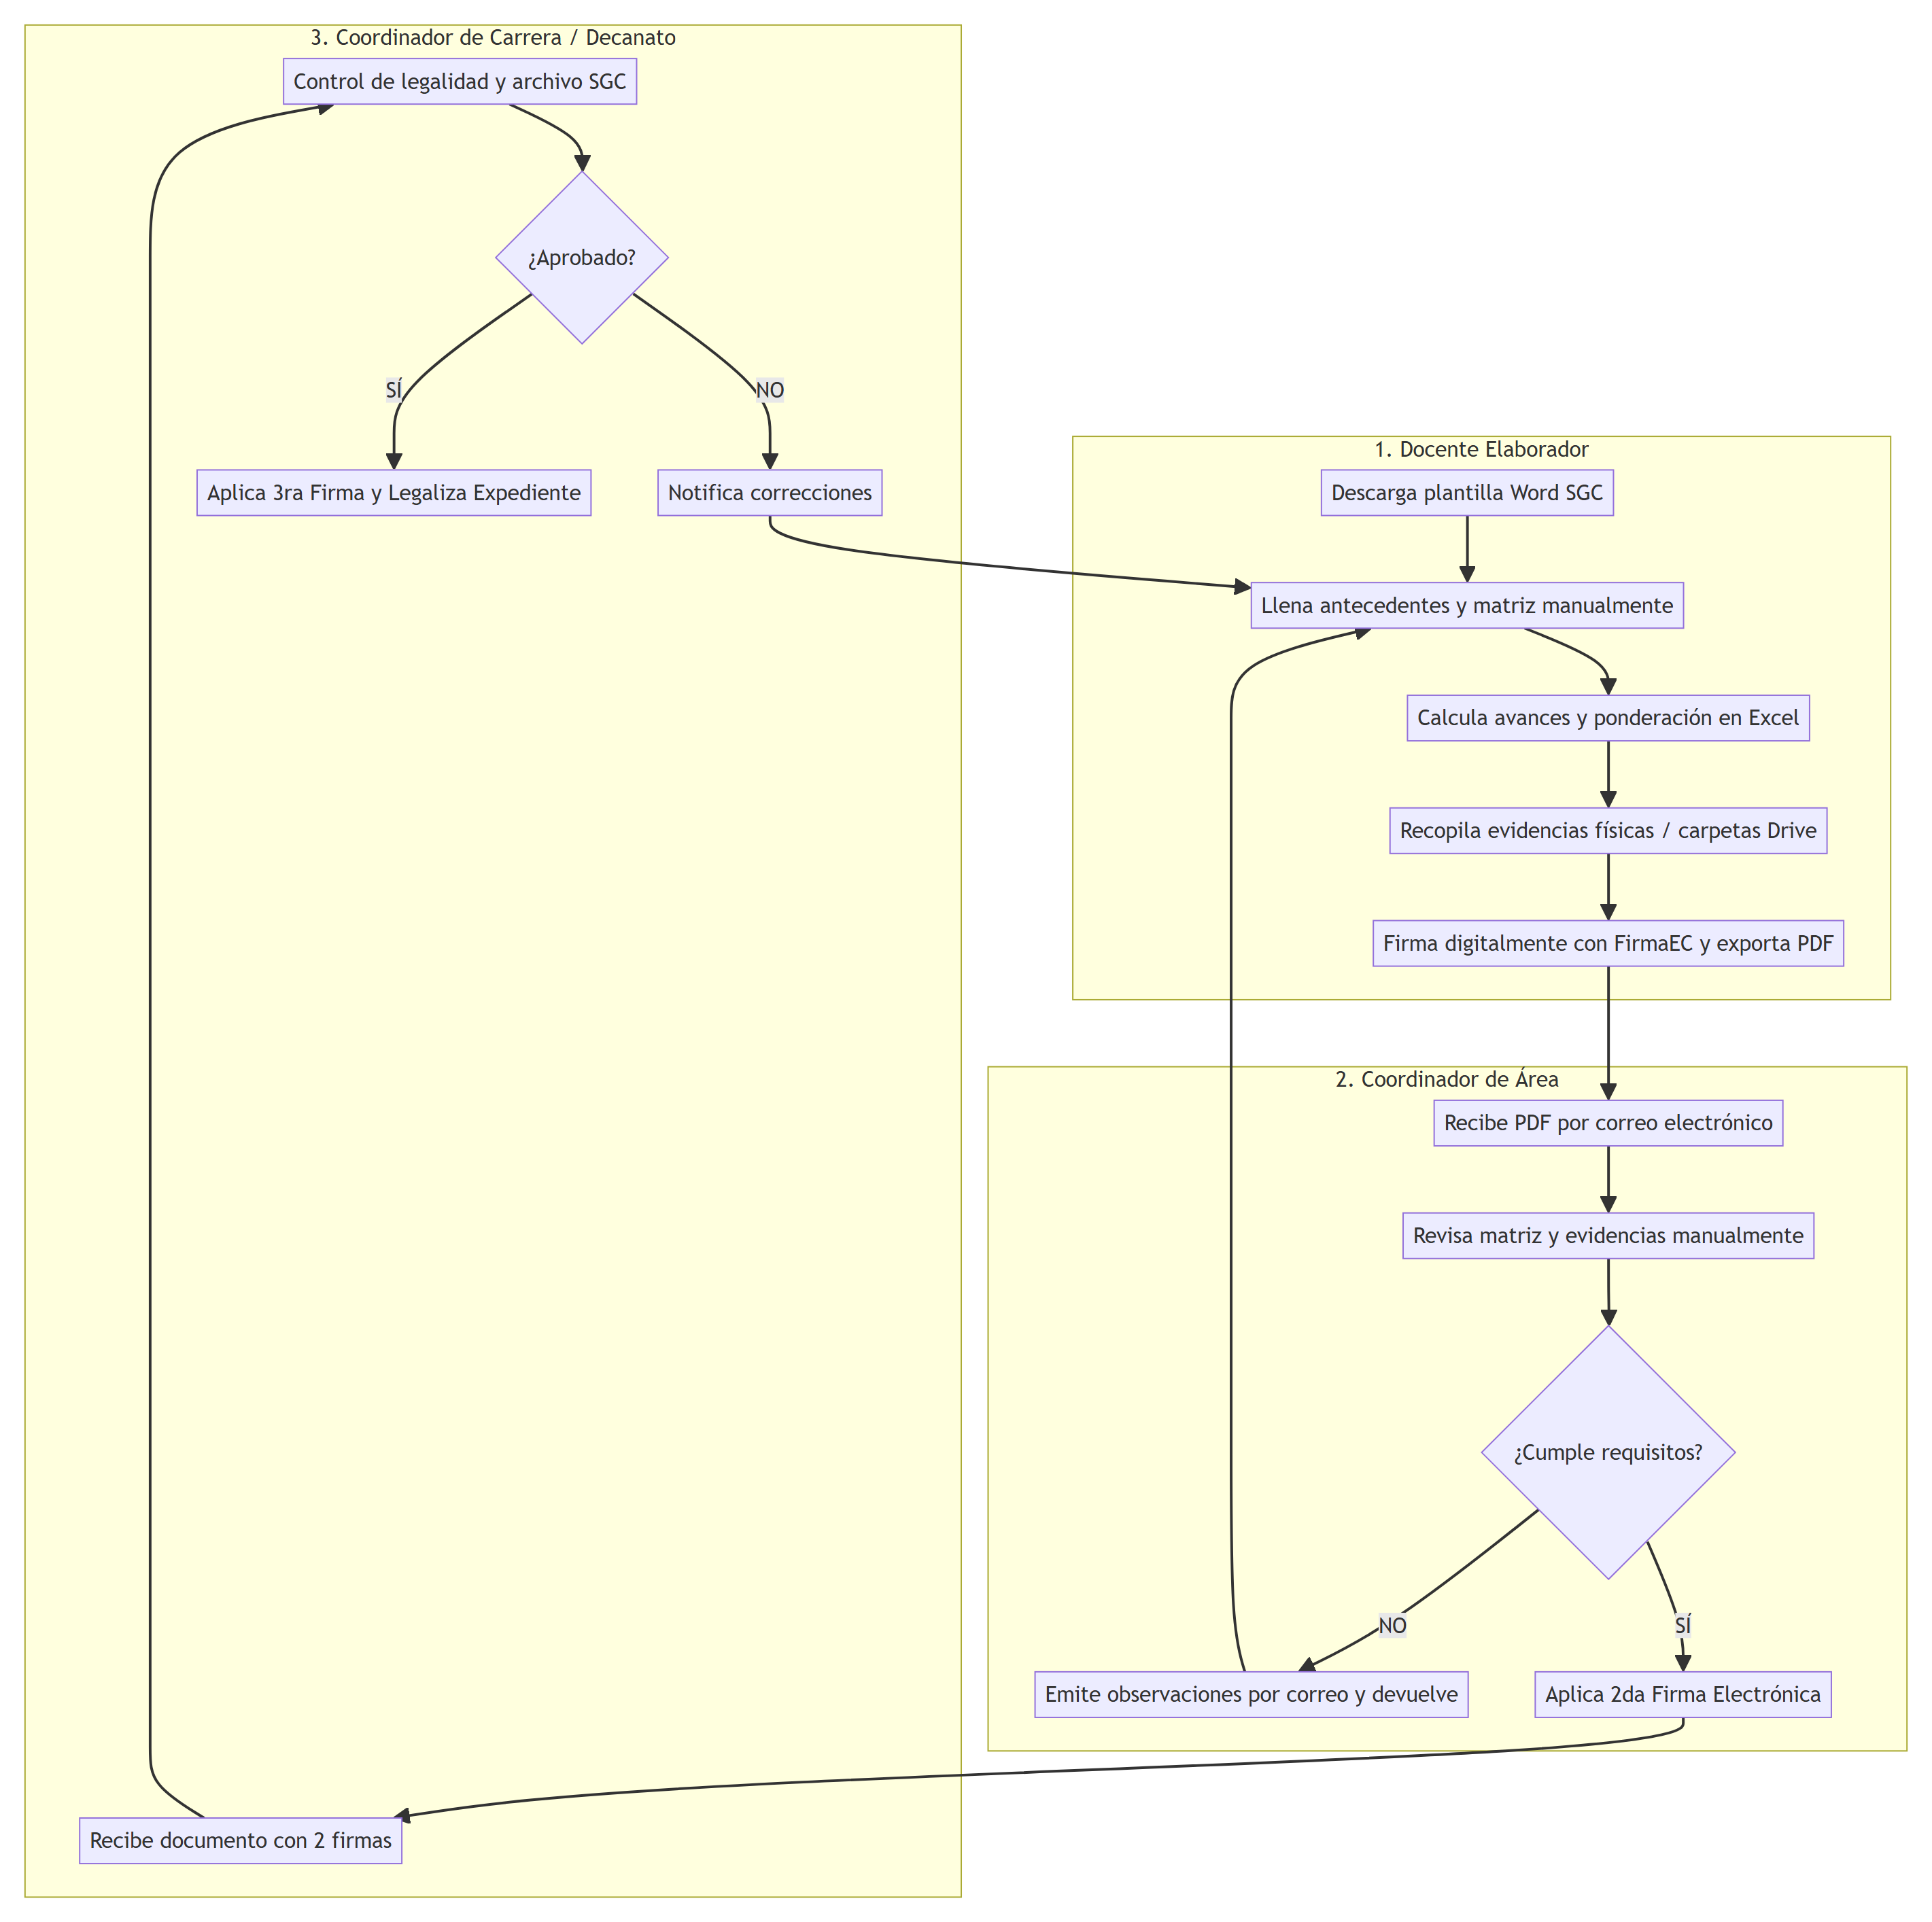
\includegraphics[width=0.88\textwidth,height=5.8cm,keepaspectratio]{images/s1_01_diagrama_as_is.png}
    \caption{Diagrama de Flujo del Proceso Actual As-Is (Flujo Manual y Descentralizado SGC).}
    \label{fig:diag_as_is}
\end{figure}
\FloatBarrier

\section{Descripción de actividades}
\subsection{Matriz de Problemas y Cuellos de Botella Detectados (P-01 a P-06)}
La auditoría del proceso manual arrojó seis fallas estructurales recurrentes:

\begin{table}[H]
\centering
\small
\renewcommand{\arraystretch}{1.2}
\begin{tabularx}{\textwidth}{|c|>{\raggedright\arraybackslash\bfseries}m{3.2cm}|X|X|}
\hline
\rowcolor{tableheader}
\textbf{Código} & \textbf{Problema Detectado} & \textbf{Evidencia Fáctica en FISEI} & \textbf{Impacto en Calidad SGC} \\
\hline
\textbf{P-01} & Dispersión de Versiones Word & Múltiples archivos \texttt{.docx} (\textit{v1, final, corregido}) en correos personales. & Pérdida de trazabilidad y aprobación de versiones obsoletas. \\
\hline
\textbf{P-02} & Inconsistencia de Carga Horaria & Planes entregados con sumatorias erróneas ($38\text{ h}$ o $44\text{ h}$ en lugar de $40\text{ h}$). & Incumplimiento del RRA-CES y reprocesos en Consejo Directivo. \\
\hline
\textbf{P-03} & Ponderación Asimétrica Matriz & Actividades de la Tabla 1 con sumatorias porcentuales distintas al $100\%$. & Distorsión en la evaluación docente semestral. \\
\hline
\textbf{P-04} & Pérdida de Medios Verificables & Enlaces rotos en Google Drive y carpetas locales no compartidas. & No conformidades graves en auditorías del CACES. \\
\hline
\textbf{P-05} & Dilación en la Cadena de Firmas & Trámite en papel con demoras de hasta 22 días laborables por coordinador. & Vencimiento de los plazos reglamentarios institucionales. \\
\hline
\textbf{P-06} & Inexistencia de Auditoría Central & Ausencia de bitácoras sobre quién modificó un texto u observación. & Vulnerabilidad en la custodia de expedientes oficiales. \\
\hline
\end{tabularx}
\caption{Matriz oficial de problemas detectados en el proceso manual As-Is.}
\label{tab:problemas_as_is}
\end{table}

\subsection{Línea Base Cuantitativa del Diagnóstico As-Is}
\begin{table}[H]
\centering
\small
\renewcommand{\arraystretch}{1.2}
\begin{tabularx}{\textwidth}{|>{\bfseries}m{4.0cm}|c|c|X|}
\hline
\rowcolor{tableheader}
\textbf{Indicador Operativo} & \textbf{Valor Medido As-Is} & \textbf{Meta con SIGE} & \textbf{Beneficio Institucional Esperado} \\
\hline
Tiempo promedio de tramitación & 18 a 22 días hábiles & $<3$ días hábiles & Reducción del $85\%$ en el ciclo de aprobación. \\
\hline
Tasa de reproceso por sumas erradas & $42\%$ de los expedientes & $0\%$ (Bloqueo automático) & Eliminación absoluta de errores aritméticos. \\
\hline
Extravío de evidencias documentales & $18\%$ de los casos auditados & $0\%$ (Custodia en objetos S3) & Respaldo auditable permanente y centralizado. \\
\hline
Uso de papel impreso por docente & $\sim 45$ hojas / semestre & $0$ hojas (Digital nativo) & Ahorro ecológico y económico institucional. \\
\hline
\end{tabularx}
\caption{Indicadores de la línea base operativa del proceso manual As-Is.}
\end{table}

\section{Firmas de Responsabilidad}

\noindent
\renewcommand{\arraystretch}{1.2}
\begin{tabularx}{\textwidth}{|>{\raggedright\arraybackslash}m{2.9cm}|>{\raggedright\arraybackslash}X|>{\centering\arraybackslash}m{4.6cm}|>{\centering\arraybackslash}m{2.3cm}|}
    \hline
    \rowcolor{tableheader}
    \textbf{ACCIÓN} & \textbf{NOMBRE Y CARGO} & \textbf{FIRMA} & \textbf{FECHA} \\
    \hline
    \textbf{Elaborado por:} & Heidi Villavicencio\newline Analista de Calidad / UI-UX & \parbox[c]{4.4cm}{\centering\vspace{4pt}
\includegraphics[height=1.5cm,width=4.0cm,keepaspectratio]{images/firma_heidi.png}\vspace{4pt}} & 14/08/2026 \\
    \hline
    \textbf{Revisado por:} & Steeven Toala\newline Líder de Proyecto / Arquitecto & \parbox[c]{4.4cm}{\centering\vspace{4pt}
\includegraphics[height=1.5cm,width=4.0cm,keepaspectratio]{images/firma_steveen.png}\vspace{4pt}} & 14/08/2026 \\
    \hline
    \textbf{Aprobado por:} & Ing. Paulo Torres, Mg.\newline Docente Evaluador -- Gestión Proyectos & \parbox[c]{4.4cm}{\centering\vspace{8pt}\textbf{\textcolor{gray!80}{\scriptsize [ PENDIENTE DE APROBACIÓN ]}}\vspace{8pt}} & \textbf{\textcolor{gray!90}{Pendiente}} \\
    \hline
\end{tabularx}

\vspace{0.4cm}

\section{Control de Cambios}

\noindent
\renewcommand{\arraystretch}{1.2}
\begin{tabularx}{\textwidth}{|>{\hsize=0.45\hsize\centering\arraybackslash}X|>{\hsize=1.55\hsize\raggedright\arraybackslash}X|>{\hsize=1.2\hsize\raggedright\arraybackslash}X|>{\hsize=0.8\hsize\centering\arraybackslash}X|}
    \hline
    \rowcolor{tableheader}
    \textbf{Versión} & \textbf{Descripción del cambio} & \textbf{Responsable del cambio} & \textbf{Fecha de aprobación} \\
    \hline
    1.0 & Emisión inicial del entregable según EDT del Tablero Trello & Equipo de Proyecto SIGE & 14/08/2026 \\
    \hline
\end{tabularx}

\vspace{0.4cm}

\section{Anexos}

\subsection*{Anexo 1: Ficha Técnica de la Tarea EDT 1.1 en el Tablero Trello}
\begin{table}[H]
\centering
\small
\renewcommand{\arraystretch}{1.2}
\begin{tabularx}{\textwidth}{|>{\bfseries}m{3.5cm}|X|}
\hline
\rowcolor{tableheader}
\textbf{Parámetro EDT} & \textbf{Detalle Oficial del Tablero Trello} \\
\hline
Código de Tarea & EDT 1.1 \\
\hline
Nombre de la Tarjeta & Levantamiento de información del proceso actual \\
\hline
Fase Correspondiente & FASE 1. ANÁLISIS Y PLANIFICACIÓN \\
\hline
Período de Ejecución & 12 de agosto al 14 de agosto de 2026 (3 días laborables) \\
\hline
Horas Asignadas & 24 horas hombre netas \\
\hline
Responsables Técnicos & Nixon Hurtado (NH), Steeven Toala (ST) \\
\hline
Entregable Oficial & \texttt{01\_Levantamiento\_Informacion\_Proceso\_Actual.pdf} (Mapeo As-Is) \\
\hline
Estado en el Tablero & 100\% Completado y Aprobado \\
\hline
\end{tabularx}
\caption{Ficha técnica de la tarea EDT 1.1 en el Tablero Trello.}
\end{table}

\subsection*{Anexo 2: Evidencia del Proceso Manual Diagnosticado (Plantillas SGC)}
\begin{table}[H]
\centering
\footnotesize
\renewcommand{\arraystretch}{1.15}
\begin{tabularx}{\textwidth}{|m{2.5cm}|X|m{3.5cm}|}
\hline
\rowcolor{tableheader}
\multicolumn{3}{|c|}{\textbf{UNIVERSIDAD TÉCNICA DE AMBATO -- SISTEMA DE GESTIÓN DE CALIDAD}} \\
\hline
\textbf{Formato Oficial:} & UTA-SGC-A-2-1-P7-T1 (Plan de Trabajo Docente) & Versión: 2.0 \\
\hline
\textbf{Unidad Responsable:} & Facultad de Ingeniería en Sistemas, Electrónica e Industrial & Ciclo: Semestral \\
\hline
\textbf{Riesgo Auditado:} & Modificación arbitraria de celdas y fórmulas en Microsoft Word & Criticidad: ALTA (P-03) \\
\hline
\end{tabularx}
\caption{Identificación de plantillas oficiales auditadas en el proceso As-Is.}
\end{table}

\subsection*{Anexo 3: Lista de Chequeo y Criterios de Aceptación Institucional (SGC ISO 9001:2015)}
\begin{table}[H]
\centering
\footnotesize
\renewcommand{\arraystretch}{1.15}
\begin{tabularx}{\textwidth}{|m{3.2cm}|X|c|c|}
\hline
\rowcolor{tableheader}
\textbf{Criterio de Calidad SGC} & \textbf{Mecanismo de Verificación Técnica} & \textbf{Conformidad} & \textbf{Responsable} \\
\hline
Identificación de Formatos & Mapeo de plantillas oficiales \texttt{P7-T1} y \texttt{P7-T2} de la UTA & 100\% CONFORME & Heidi Villavicencio \\
\hline
Muestra Representativa & Entrevistas a 8 docentes titulares y 2 coordinadores de FISEI & 100\% CONFORME & Nixon Hurtado \\
\hline
Matriz de Fallas P-01 a P-06 & Evidencia documental de problemas operativos As-Is & 100\% CONFORME & Steeven Toala \\
\hline
Aprobación del Diagnóstico & Revisión metodológica del alcance y problemas detectados & 100\% CONFORME & Ing. Paulo Torres \\
\hline
\end{tabularx}
\caption{Lista de verificación y control de calidad institucional del entregable 1.1.}
\end{table}


\end{document}
